\documentclass{article}
\usepackage{graphicx} % Required for inserting images
\usepackage{amssymb}
\usepackage{listings}
\usepackage{amsmath} 
\usepackage{algorithm}
\usepackage{algpseudocode}

\newcommand{\graph}{\mathcal{G}}

\title{hetFL}
\author{shamsiiat.abdurakhmanova }
\date{\today}

\begin{document}

\maketitle

\section{Numerical experiments}

\subsection{Datasets}

\subsubsection{Synthetic Dataset}

Experiments were performed on a synthetic dataset whose empirical graph $\mathcal {G}$ is partitioned into 3 equal-sized clusters $\mathcal{P} = \{\mathcal{C}^{(1)}, \mathcal{C}^{(2)}, \mathcal{C}^{(3)}\}$, with $|\mathcal{C}^{(1)}|=|\mathcal{C}^{(2)}|=|\mathcal{C}^{(3)}|$. We denote the cluster assignment of node $i \in \mathcal{V}$ by ${c}^{(i)} \in \{1,2,3\}$. 

For experiments where graph connectivity is known, the edges in $\mathcal {G}$  are generated via realizations of independent binary random variables ${b}_{i,{i}^{'}} \in \{0,1\}$. These random variables are indexed by pairs $i,{i}^{'}$ of nodes that are connected by an edge $\{i,{i}^{'}\} \in \mathcal{E}$ if and only if ${b}_{i,{i}^{'}}=1$. \\
Two nodes in the same cluster are connected with probability $Prob\{{b}_{i,i'}=1\} :={p}_{in}$ if nodes $i,i'$ belong to the same cluster. In contrast, $Prob\{{b}_{i,{i}^{'}}=1\} :={p}_{out}$ if nodes $i,{i}^{'}$ belong to different clusters. Every edge in  $\mathcal {G}$ has the same weight, ${A}_{e}=1$ for all $e \in \mathcal{E}$.

Each node $i \in \mathcal {V}$ of the empirical graph $\mathcal {G}$ holds a local dataset $\mathcal {D}^{(i)}$ of the form $\mathcal {D}^{(i)} := \{ (\mathbf{x}^{(i,1)}, {y}^{(i,1)}), ..., (\mathbf{x}^{(i,{m}_{i})}, {y}^{(i,{m}_{i})}) \}$. Thus, dataset $\mathcal {D}^{(i)}$ consist of ${m}_{i}$ data points, each characterized by a feature vector $\mathbf{x}^{(i,r)} \in \mathbb{R}^{d}$ and scalar label ${y}^{(i,r)}$, for $r=1,...,{m}_{i}$. The feature vectors $\mathbf{x}^{(i,r)} \sim \mathcal{N}(\mathbf{0},\mathbf{I}_{d \times d})$, are drawn i.i.d. from a standard multivariate normal distribution. 

The labels of the data points are generated by a noisy linear model
\begin{equation}
{y}^{(i,r)} = (\mathbf{w}^{(i)})^T\mathbf{x}^{(i,r)} + {\varepsilon}^{(i,r)}
\end{equation}

The noise ${\varepsilon}^{(i,r)} \sim \mathcal{N}(0, 1)$, for $i \in \mathcal{V}$ and $r=1,..,{m}_{i}$, are i.i.d. realizations of a normal distribution. The true underlying vector $\mathbf{\overline{w}}^{(i)} \sim \mathcal{N}(\mathbf{0},\mathbf{I}_{d \times d})$ is drawn from a standard normal distribution and is the same for nodes from the same cluster, i.e. $\mathbf{\overline{w}}^{(i)}=\mathbf{\overline{w}}^{({i'})}$ if ${c}^{(i)}={c}^{({i'})}$.

(!!! Not relevant if we only interested in weight vector est.error!!!) Datasets are divided into training and validation subsets by using resampling with replacement. The size of the validation subset is ${m}^{(val)}_{i}=100$. 

\subsubsection{Shared Dataset}

The dataset $\mathcal{D}^{(test)} := \{\mathbf{x}^{(i)}, ..., \mathbf{x}^{(m')} \}$ consist of only feature vectors (no labels), where feature vector is sampled as $\mathbf{x}^{(r)} \sim \mathcal{N}(\mathbf{0},\mathbf{I}_{d \times d})$.
Predictions on $\mathcal{D}^{(test)}$ are shared across all nodes. The size of the dataset is $m'=100$. 

\subsection{Experiments}

\subsubsection{Synthetic Dataset, linreg model, graph is known}

In these experiments empirical graph $\mathcal{G}$ consist of $N=150$ nodes partitioned into three clusters ($|\mathcal{C}^{(i)}|=50$). Two nodes in the same cluster are connected with probability ${p}_{in}=0.8$ if nodes $i,{i}^{'}$ belong to the same cluster and ${p}_{out}=0.2$ if nodes $i,{i}^{'}$ belong to different clusters. 

Each node $i \in \mathcal {V}$ of the empirical graph $\mathcal {G}$ holds a local dataset $\mathcal{D}^{(i)}$ consisting of ${m}_{i}$ data points, each characterized by a feature vector $\mathbf{x}^{(i,r)} \in \mathbb{R}^{d}$ and scalar label ${y}^{(i,r)}$, for $r=1,...,{m}_{i}$, where $d=10$.
The sample size of the shared dataset $\mathcal{D}^{(test)}$ is $m'=100$.

To learn the local parameters $\mathbf{w}^{(i)}$, we use Algorithm 1. FedRelax Least-Squares Regression with local loss 

\begin{equation}
{L}_{(i)}({h}^{(i)}) = \frac{1}{{m}_{i}} \sum_{r=1}^{{m}_{i}}\left({y}^{(i,r)} - {h}^{(i)}(\mathbf{x}^{(i,r)}) \right)^2
\end{equation}

and  regularizer 

\begin{equation}
\frac{\lambda}{2m'} \sum_{{i}^{'} \in {\mathcal V}} {A}_{i,{i}^{'}} \sum_{r=1}^{m'} \left({h}^{(i)}(\mathbf{x}^{(r)}) - {h}^{({i}^{'})}(\mathbf{x}^{(r)}) \right)^2
\end{equation}

\newpage
\begin{algorithm}[htbp]
	\caption{FedRelax Least-Squares Regression (Adjacency matrix is known)}
	\label{alg_X_param}
	{\bf Input}: empirical graph $\graph$ with edge weights $A_{ij}$; 
	local loss $L_{(i)}{(\cdot)}$; shared dataset $D^{(test)} = \{\mathbf{x}^{(1)}, ..., \mathbf{x}^{(m')}\}$; GTV parameter $\lambda$; \\
	{\bf Initialize}: $k:=0;$ predictions on shared set $\{\widehat{h}_{0}^{(i)}(\mathbf{x})\}_{\mathbf{x} \in \mathcal{D}^(test)}:=0$ for all nodes $i \in \mathcal{V}$.
	\begin{algorithmic}[1]
		\While{stopping criterion is not met do}
		\For{all nodes $i \in \mathcal{V}$ in parallel}
		\State share predictions $\{\widehat{h}_{k}^{(i)}(\mathbf{x})\}_{\mathbf{x} \in \mathcal{D}^(test)}$, 
		with neighbours $i' \in \mathcal{N}^{(i)}$ 
		\State update local hypothesis $\widehat{h}_{k}^{(i)}$ by
            \begin{multline*}
            \widehat{h}_{k+1}^{(i)} \in  \arg \min_{h^{(i)} \in \mathcal{H}^{(i)}} 
            \biggl[ \frac{1}{m_i}  \sum_{r=1}^{m_i} \biggl( y^{(i,r)} - h^{(i)}(\mathbf{x}^{(i,r)})  \biggr)^2 + \\
            \frac{\lambda}{m'} \sum_{i' \in \mathcal{N}^{(i)}}A_{i,i'}\sum_{r=1}^{m'} \biggl( h^{(i)}(\mathbf{x}^{(r)}) - \widehat{h}_{k}^{(i')}(\mathbf{x}^{(r)}) \biggr)^2 \biggr]
            \end{multline*}
		\EndFor
		\State $k := k+1$
		\EndWhile
	\end{algorithmic}
\end{algorithm}

For the experiment we use linear model implemented with pytorch (no bias, optimizer SGD learning rate 0.01). We try different local dataset sizes $m_i =$ \{2, 3, 5, 10, 20\} and regularization strength $\lambda =$ \{0, 1, 5\}. Tried ratio $|\mathcal{C}^{(i)}|m_i / d = \{1, 1.5, 2.5, 5, 10\}$ or $d / m_i = \{5, 3.3, 2, 1, 0.5\}$ 

As stopping criterion in Algorithm 1, we use a fixed number of R = 2000 iterations. 
For pytorch models one iteration is equivalent to one gradient step.

The results of the experiments is depicted in Figure 1 as the plot of mean estimation error (mean over 10 repetitions of the experiment for each pair of $\{\lambda, m_i \}$). 
\begin{equation} \label{eq:4}
\frac{1}{N} \sum_{i=1}^{N} ||\mathbf{\overline{w}}^{(i)} - \mathbf{\widehat{w}}^{(i)}||^2_2
\end{equation}

The 2nd row of the Figure 1 shows estimation error scaled by estimation error of the "pooled" model (model trained on all datasets belonging to the same cluster).


On each repetition new local $\mathcal{D}^{(i)}$ (new realizations of feature vectors and cluster-specific weights are drawn) and shared $\mathcal{D}^{(test)}$ (new realizations of feature vectors are drawn) datasets were generated. The shaded region is $\pm$ one standard deviation.  

\begin{figure}[h]
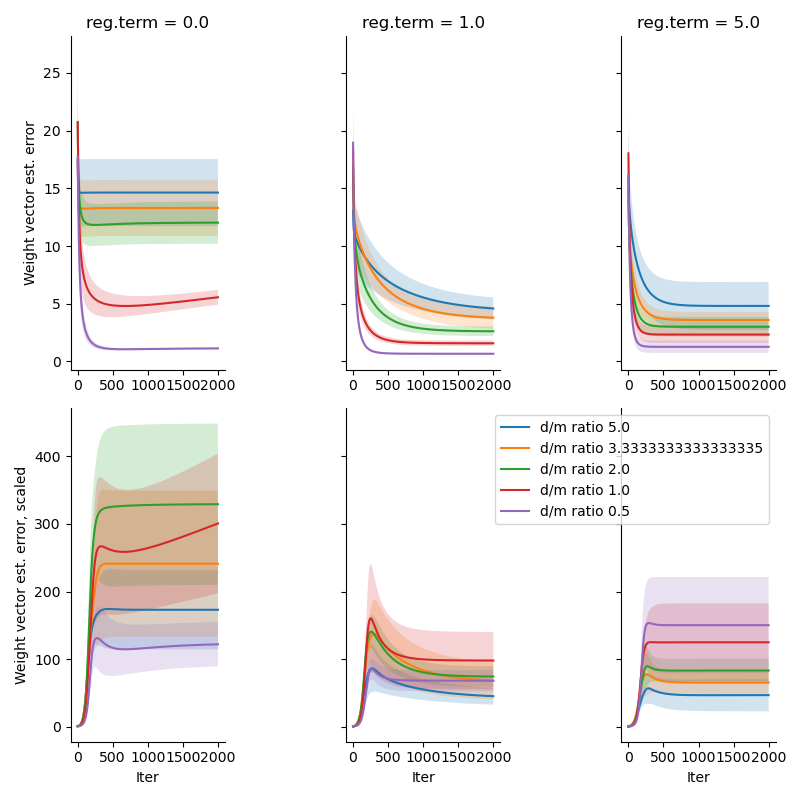
\includegraphics[width=10cm]{Linreg_Torch_637015_est_error.png}
\caption{Algorithm 1 weight vector estimation error. Subplots corresponds to different regularization parameter values and lines correspond to different ratio d/m of a feature vector and local dataset size.}
\end{figure}

We can see from the Figure 1, that adding penalty term helps to converge to the true weight vector, the effect more pronounced for the larger d/m ratio. Large values of $\lambda$ leads to sightly higher and noisier weight error estimates, but faster convergence (subplot with $\lambda=5$). 

\newpage
\subsubsection{Sanity check}
Below I do sanity check for the case where $p_{in}=1$ and $p_{out}=0$. The expected estimation error (eq.\ref{eq:4}) is  

\begin{equation}
\begin{split}
E_{est} & = \mathop{\mathbb{E}}\{||\mathbf{\overline{w}} - \mathbf{\widehat{w}}||^2_2\} \\
& = \mathop{\mathbb{E}}\{||\mathbf{\widehat{w}}- \mathop{\mathbb{E}}\{\mathbf{\widehat{w}}\}||^2_2\} + 
\mathop{\mathbb{E}}\{||\mathbf{\overline{w}} - \mathop{\mathbb{E}}\{\mathbf{\widehat{w}}\}||^2_2\}
\end{split}
\end{equation}

The first component represents the (expected) variance of the learnt parameter vector $\mathbf{\widehat{w}}$. The second component is referred to as a bias term. It can be shown that the variance term is

\begin{equation} 
V = \mathop{\mathbb{E}}\{||\mathbf{\widehat{w}}- \mathop{\mathbb{E}}\{\mathbf{\widehat{w}}\}||^2_2\} = \frac{(B^2 + \sigma^2)d}{m-d-1}
\end{equation}

E.g. for the case $B^2=0, \sigma^2=1, d=10, m=20, |\mathcal{C}^{(i)}|=50$ variance term is $10/(20-1-1)  \approx 1.11$ for a local model and  $10/(20*50-10-1)  \approx 0.01$ for pooled model.
For $\lambda = 0, p_{in}=1$ and $p_{out}=0$ the scaled estimated error is $\frac{E_{est}}{E_{est\_pooled}} = 1.11/0.01 \approx 111$. For the large values of $\lambda$ the ratio is expected to be close to 1.

\begin{figure}[h]
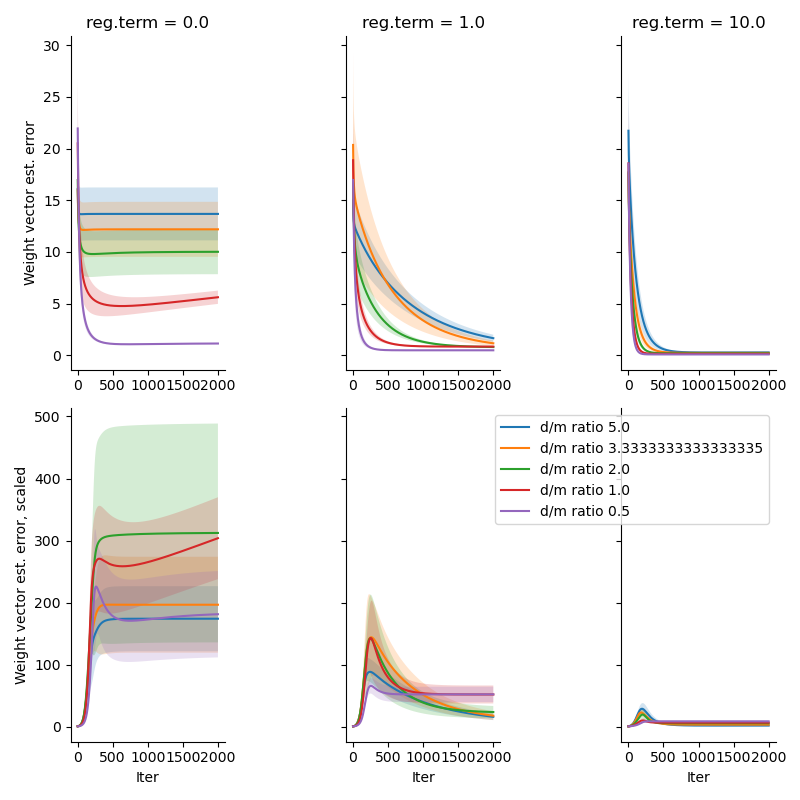
\includegraphics[width=10cm]{Linreg_Torch_594391_est_error.png}
\caption{Algorithm 1 for params $p_{in}=1, p_{out}=0$}
\end{figure}

From the Figure 2 we can see that according to numerical experiments $\frac{E_{est}}{E_{est\_pooled}} \approx 180$ for the $m=20$, which is somewhat higher than estimate $\approx 111$, but of the same order. Increasing $\lambda$ leads to decrease of estimation error ($\approx 9$ according to numerical experiments).


\newpage
\subsubsection{Synthetic Dataset, linreg model, graph is not known}

The variation of Algorithm 1, Algorithm 2a, is used for the case when the graph connectivity is not known. In Algorithm 2a we start with adjacency matrix set to zero and on each iteration we add $p$ links between nodes with smallest discrepancy in predictions on the shared test set $\mathcal{D}^{(test)}$. Thus, on each iteration each node's degree is either increasing or stays unchanged (but not decreasing). See resulting plots in Fig.3 and 4.

\begin{algorithm}[htbp]
	\caption{FedRelax Least-Squares Regression (Adjacency matrix is not known, degree of the node is not fixed)}
	\label{alg:algorithm1}
	{\bf Input}: empirical graph $\graph$; 
	local loss $L_{(i)}{(\cdot)}$; shared dataset $D^{(test)} = \{\mathbf{x}^{(1)}, ..., \mathbf{x}^{(m')}\}$; GTV parameter $\lambda$; \\
	{\bf Initialize}: $k:=0; A:=0;$ predictions on shared set $\{\widehat{h}_{0}^{(i)}(\mathbf{x})\}_{\mathbf{x} \in \mathcal{D}^(test)}:=0$ for all nodes $i \in \mathcal{V}$.
	\begin{algorithmic}[1]
		\While{stopping criterion is not met do}
		\For{all nodes $i \in \mathcal{V}$ in parallel}
		\State share predictions $\{\widehat{h}_{k}^{(i)}(\mathbf{x})\}_{\mathbf{x} \in \mathcal{D}^(test)}$, 
		with neighbours $i' \in \mathcal{N}^{(i)}$ 
		\State update local hypothesis $\widehat{h}_{k}^{(i)}$ by
            \begin{multline*}
            \widehat{h}_{k+1}^{(i)} \in  \arg \min_{h^{(i)} \in \mathcal{H}^{(i)}} 
            \biggl[ \frac{1}{m_i}  \sum_{r=1}^{m_i} \biggl( y^{(i,r)} - h^{(i)}(\mathbf{x}^{(i,r)})  \biggr)^2 + \\
            \frac{\lambda}{m'} \sum_{i' \in \mathcal{N}^{(i)}}A_{i,i'}\sum_{r=1}^{m'} \biggl( h^{(i)}(\mathbf{x}^{(r)}) - \widehat{h}_{k}^{(i')}(\mathbf{x}^{(r)}) \biggr)^2 \biggr]
            \end{multline*}
        \EndFor
        \For{all nodes $i \in \mathcal{V}$ in parallel}
        \State Add neighbours (edges) for the node $i$ by selecting $p$ nodes $i' \in \mathcal{V}$ with smallest values of
             \begin{align}
                \frac{1}{m'} \sum_{r=1}^{m'} \biggl( \widehat{h}_{k+1}^{(i)}(\mathbf{x}^{(r)}) - \widehat{h}_{k+1}^{(i')}(\mathbf{x}^{(r)}) \biggr)^2 
             \end{align}
        \State Set $A_{i,i'} = 1$ for these $p$ nodes (with smallest discrepancy in prediction on the test set $\mathcal{D}^{(test)}$).
        \EndFor
        \State $k := k+1$
		\EndWhile
	\end{algorithmic}
\end{algorithm}

\begin{figure}[h]
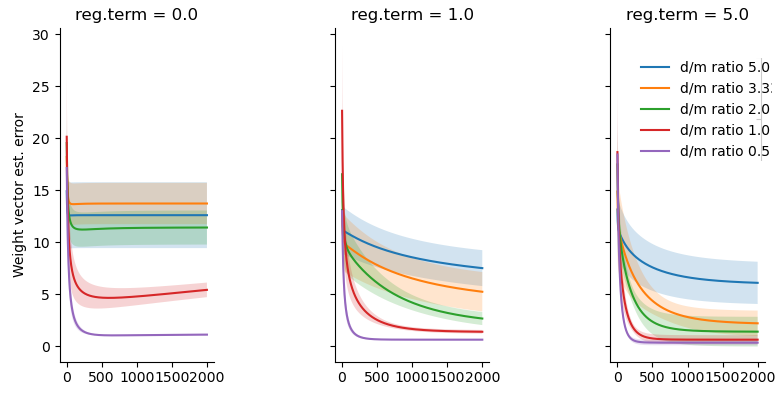
\includegraphics[width=10cm]{Linreg_Torch_665413_est_error_Algo2a_nn10.png}
\caption{Algorithm 2a. Estimated error for the weight vector with parameter p=10}
\end{figure}

\begin{figure}[h]
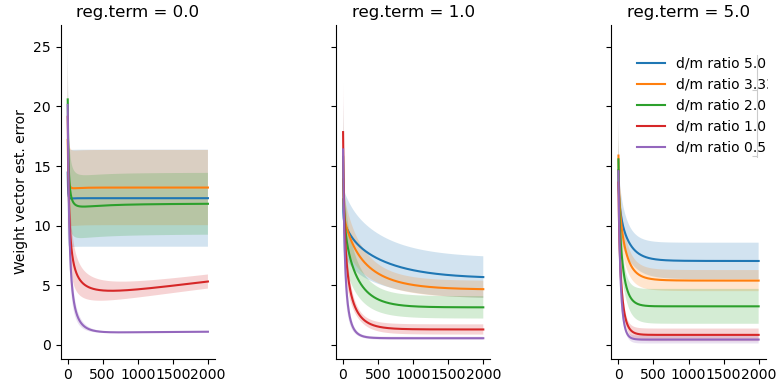
\includegraphics[width=10cm]{Linreg_Torch_672336_est_error_Algo2a_nn50.png}
\caption{Algorithm 2a. Estimated error for the weight vector with parameter p=50.}
\end{figure}

\newpage
In another variation, Algorithm 2b, we set adjacency matrix to zero on each iteration and then add $p$ links between nodes with smallest discrepancy in predictions on the shared test set $\mathcal{D}^{(test)}$. Thus, the degree of  a node is fixed to $p$. See resulting plot in Fig.5.

\begin{figure}[h]
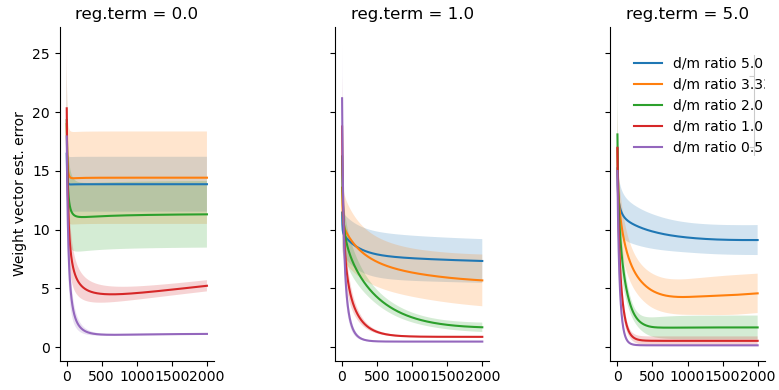
\includegraphics[width=10cm]{Linreg_Torch_673711_est_error_algo2b_nn50.png}
\caption{Algorithm 2b. Estimated error for the weight vector with parameter p=50.}
\end{figure}

\begin{algorithm}[htbp]
	\caption{FedRelax Least-Squares Regression (Adjacency matrix is not known, n.o. neib. is fixed)}
	\label{alg_X_param}
	{\bf Input}: empirical graph $\graph$; 
	local loss $L_{(i)}{(\cdot)}$; shared dataset $D^{(test)} = \{\mathbf{x}^{(1)}, ..., \mathbf{x}^{(m')}\}$; GTV parameter $\lambda$; \\
	{\bf Initialize}: $k:=0; A:=0;$ predictions on shared set $\{\widehat{h}_{0}^{(i)}(\mathbf{x})\}_{\mathbf{x} \in \mathcal{D}^(test)}:=0$ for all nodes $i \in \mathcal{V}$.
	\begin{algorithmic}[1]
		\While{stopping criterion is not met do}
		\For{all nodes $i \in \mathcal{V}$ in parallel}
		\State share predictions $\{\widehat{h}_{k}^{(i)}(\mathbf{x})\}_{\mathbf{x} \in \mathcal{D}^(test)}$, 
		with neighbours $i' \in \mathcal{N}^{(i)}$ 
		\State update local hypothesis $\widehat{h}_{k}^{(i)}$ by
            \begin{multline*}
            \widehat{h}_{k+1}^{(i)} \in  \arg \min_{h^{(i)} \in \mathcal{H}^{(i)}} 
            \biggl[ \frac{1}{m_i}  \sum_{r=1}^{m_i} \biggl( y^{(i,r)} - h^{(i)}(\mathbf{x}^{(i,r)})  \biggr)^2 + \\
            \frac{\lambda}{m'} \sum_{i' \in \mathcal{N}^{(i)}}A_{i,i'}\sum_{r=1}^{m'} \biggl( h^{(i)}(\mathbf{x}^{(r)}) - \widehat{h}_{k}^{(i')}(\mathbf{x}^{(r)}) \biggr)^2 \biggr]
            \end{multline*}
		\EndFor
        \For{all nodes $i \in \mathcal{V}$ in parallel}
        \State \textbf{Init a new adjacent matrix A (all zeros)}
        \State Add neighbours for the node $i$ by selecting $p$ nodes $i' \in \mathcal{V}$ with smallest values of
             \begin{align}
                \frac{1}{m'} \sum_{r=1}^{m'} \biggl( \widehat{h}_{k+1}^{(i)}(\mathbf{x}^{(r)}) - \widehat{h}_{k+1}^{(i')}(\mathbf{x}^{(r)}) \biggr)^2 
             \end{align}
        \State Set $A_{i,i'} = 1$ for these $p$ nodes (with smallest discrepancy in prediction on the test set $\mathcal{D}^{(test)}$).
        \EndFor
        \State $k := k+1$
		\EndWhile
	\end{algorithmic}
\end{algorithm}

\end{document}
